\documentclass[conference]{IEEEtran}
\usepackage{float}
\usepackage{graphicx}
\usepackage{mathtools}
\usepackage{amssymb}
\usepackage{amsthm}

\begin{document}

\title{Device-Agnostic Wi-Fi Fingerprint Positioning for Consumer Applications}

\author{\IEEEauthorblockN{Daniel Griffin}
\IEEEauthorblockA{Tufts University}
\and
\IEEEauthorblockN{Hunter Wapman}
\IEEEauthorblockA{Tufts University}
\and
\IEEEauthorblockN{Brett Fischler}
\IEEEauthorblockA{Tufts University}
\and
\IEEEauthorblockN{Tyler Lubeck}
\IEEEauthorblockA{Tufts University}
\and
\IEEEauthorblockN{Mai Vu, PhD}
\IEEEauthorblockA{Tufts University}}

\maketitle

\begin{abstract}
There is a growing need to position wireless devices in the real world for applications such as navigation, emergency location services, and contextual advertisements. Though GPS and the cellular network provide viable outdoor accuracy, these approaches are unsuited for indoor positioning because of non-Line of Sight environment. We propose a high-accuracy Wi-Fi Fingerprint-based indoor positioning system ideal for consumer applications. This system can be implemented in any Wi-Fi-enabled environment without modifying the site. We propose several optimized distance metrics as well as two novel environment-based methods, a density penalty factor and a floor preprocessing technique, to improve the accuracy of the Weighted K-Nearest Neighbor algorithm. Our implementation requires only thirteen minutes of site-survey time per 100m$^2$ and has an average positioning accuracy of 2.66m, which is sufficient for most practical applications.
\end{abstract}

\IEEEpeerreviewmaketitle

\section{Introduction}
As the number of wireless computing devices grows, there is a corresponding need to integrate these devices with the physical world to provide contextually relevant services. The device's position can be particularly valuable to a consumer or business. A consumer could locate a friend within a building; a business could provide location-dependent advertisements.\\
\indent Global Navigation Satellite Systems (GNSS), such as GPS, achieve acceptable accuracy outdoors, but perform poorly indoors, under No-Line of Sight (No-LoS) conditions  \cite{Lakmali}. GNSS relies on LoS conditions to determine the position of a wireless device through triangulation or trilateration. The lack of LoS conditions indoors poses a serious challenge to these methods, requiring specialized hardware to achieve acceptable accuracy \cite{Liu}. \\
\indent Most indoor positioning systems rely on Wi-Fi networks, as they are widely available and supported by most consumer hardware. This availability makes Wi-Fi networks the lowest cost option for positioning, since the required infrastructure already exists. When using Wi-Fi for positioning, there are two viable approaches: site-simulation using a signal-propagation model \cite{Kokkinis}, and manual site-survey \cite{Chaudhuri}. Site-simulation allows for rapid site integration but requires prior knowledge of the location of wireless access points (WAPs). Conversely, site-survey makes no assumptions about the environment but requires more time to integrate each site. \\
\indent Several indoor positioning systems have been successfully implemented. The RADAR positioning system utilizes fingerprinting, achieving an average accuracy of 3m to 5m within a controlled environment \cite{Bahl}. Another method, based on site-simulation, achieves an average accuracy of 1.46m by incorporating additional building information \cite{Kokkinis}. While these systems are successful, they were implemented in highly-controlled environments using site information that is not commonly available in commercial settings.\\
\indent We design and implement an indoor positioning system using Wi-Fi signals based on the site-survey method for use within a fixed commercial environment. Our system uses the nearest neighbor algorithm to estimate the position of smart phone devices. We further propose several novel distance metrics, as well as two environment-based algorithm augmentations to improve accuracy. Our system requires a low site-survey time and achieves a competitive level of accuracy, despite using consumer hardware.\\
\indent This paper is organized as follows: we first state the aims of our work, followed by a discussion of how Fingerprints (FP) are recorded and how the FP database is created. We then discuss our positioning algorithm, describing the distance metrics and algorithm refinements, before presenting the performance of our implementation and comparing it against other systems. Finally, we discuss areas for future work.

\section{Indoor Positioning System}
The basic requirements for this indoor positioning system are to provide room-level precision, widespread coverage, and real-time feedback. An indoor positioning system for use in commercial settings must additionally be usable on a variety of devices, serve multiple users simultaneously, and scale with a large user base. Further, the system must function without extensive knowledge of or modifications to the site, and must be cheap to implement. \\
\indent We design and implement an indoor positioning system which demonstrates the viability of an indoor positioning application in an environment facing constraints similar to the commercial setting described above. Our approach uses Received Signal Strength (RSS) measurements from a Wi-Fi network to position a Wireless Device (WD). RSS measurements can be effectively used for wireless indoor positioning by utilizing a Fingerprint (FP) map and a classifying algorithm. Each FP has a unique position on a floor plan, as well as a set of paired MAC addresses and RSS values.\\
\indent Our application follows the client-server model, which uses a single central server to serve a large number of clients \cite{Fielding}. The server manages the map database and uses HTTP to respond with our position estimation upon receiving a request containing an FP set. This approach is hardware-agnostic, easily scales to multiple users, and also allows simultaneous FP recording on multiple WDs, significantly speeding up the site-survey process.\\ 
\indent We provide quantitative analyses of how different decisions, such as the number of scans and floor-detection preprocessing, affected the runtime and accuracy of our positioning application. Our application can be modified for higher accuracy at the cost of increasing mapping time, and vice versa.

\begin{figure}[t!]
  \centering
    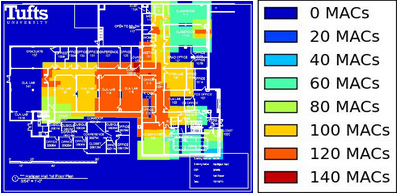
\includegraphics[width=0.5\textwidth]{APContour}
    \caption{Visible unique MAC addresses in accessible areas on the first floor of Halligan Hall}
    \label{fig:visible_unique_macs}
\end{figure}


\begin{figure}[t!]
  \centering
    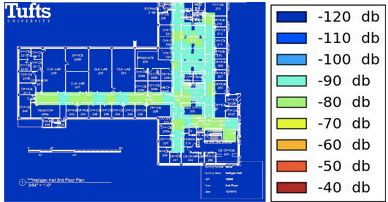
\includegraphics[width=0.5\textwidth]{dbContour}
   \caption{Average RSS contour map in accessible areas on the second floor of Halligan Hall}
   \label{fig:rss_contour_map}
\end{figure}

\section{Floor Mapping}
We now describe the building environment and discuss the methods used to generate the FP database.
\subsection{Building Environment}
We mapped two floors of Halligan Hall, the Computer Science and Electrical Engineering building at Tufts University. The average accessible area of each floor is 600m$^2$. The floor plans were available, but the locations of wireless access points were not disclosed. Furthermore, there are several inaccessible areas in the building, such as restrooms and offices. As such, this building models the commercial constraints described above. Since the location of the access points was unknown, contour maps were generated in order to examine the number of unique MAC addresses visible at each accessible location, as well as the average RSS values. Unsurveyed areas were assumed to have 0 visible MAC addresses and have an average RSS of -120 dB. 

We performed the mapping of both visible MAC addresses and average RSS values on all floors. Figure \ref{fig:visible_unique_macs} shows the MAC addresses visible on the first floor of Halligan Hall, while Figure \ref{fig:rss_contour_map} shows the average RSS values on the second floor of Halligan Hall.

\subsection{Fingerprint Logging Methodology}

\begin{figure}[t!] 
  \centering
    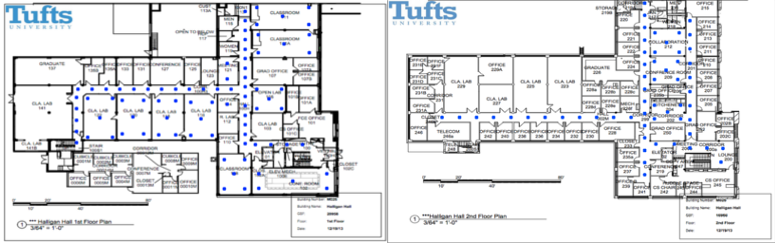
\includegraphics[width=0.5\textwidth]{floorImage.png}
     \caption{Mapped locations in Halligan Hall on both floors}
     \label{fig:mapped_positions}
\end{figure}


To build the FP database, the average of thirty RSS scans is logged for each mapped location, indicated in Figure \ref{fig:mapped_positions}. These locations were chosen manually through an examination of the floor plans and knowledge of the facility's accessibility. Each recording is stored as four values: a MAC address, an average RSS value, a standard deviation, and an association with a location on a map. The recordings were taken at locations estimated with reference to the points in Figure \ref{fig:mapped_positions}.\\
\indent In deciding the number of scans for each chosen location, we consider three factors: time, RSS precision, and MAC address coverage. We test a sample of scan values between one and one hundred using a single WD. The average Euclidean distance between each of the scans was under 1 dB when using $\sigma_E$ (Equation \ref{eq:euclidean_ideal}). Given the similarity of RSS values independent of the number of scans per location, we focus on the remaining two factors: time and MAC coverage. 


\begin{table}[!t]
\renewcommand{\arraystretch}{1.3}
\caption{Floor Recording Times (average 1.5 sec/scan)}
\label{tab:table_floor_times}
\centering
\resizebox{\columnwidth}{!}{
\begin{tabular}{|c|c|c|c|c|c|}
\hline
Scans per Position & 2 & 10 & \textbf{30} & 60 & 100 \\
\hline
Scan Time per Floor (Hours)               & 0.24   & 1.2     & \textbf{3.5}     & 7.0      & 12\\
\hline
\end{tabular}
}
\end{table}

\indent Increasing the number of scans improves MAC coverage, but involves a time tradeoff, as scanning is the most time-consuming part of site survey. Different WDs have dramatically different scan times, ranging from 0.20 to 2.0 seconds per scan. Table \ref{tab:table_floor_times} lists the approximate time to record a floor for each number of scans, assuming the worst-case scan time. The number of locations on each floor is based on the average number of locations facing only one direction.

\indent We choose a number of scans for site surveying which balances MAC coverage against worst-case device runtime. Given the similarity of MAC coverage, as shown in Table \ref{tab:MAC_accuracy}, for 30 scans and 100 scans and the runtimes of each, we opt for 30 scans.\\
\indent When recording the FP database, four devices were utilized: the HTC One m7 (Wi-Fi: IEEE 802.11 a/ac/b/g/n), LG Nexus 5  (Wi-Fi: IEEE 802.11 a/ac/b/g/n), Samsung Galaxy S3 (Wi-Fi: Wi-Fi 802.11 a/b/g/n), and Samsung Galaxy Nexus (Wi-Fi: IEEE 802.11 a/b/g/n). Because of different phones' hardware and processing capabilities, the average difference between each phone's recording of the same physical location was 6.3 dB, using $\sigma_E$ (Equation \ref{eq:euclidean}). This value is notably high in comparison to the average difference of 1.7 dB between four surveys made using the same phone. Despite this inconsistency among devices, our final application provides acceptable levels of accuracy. This decision to use multiple devices reflects our desire to build a device-agnostic system. Further, supporting a variety of device types significantly speeds up the mapping process, as parallel mapping is possible.\\
\indent A final consideration is the direction of the recording device as direction significantly effects measurements \cite{Sayad}. We found an average difference of 4.0 dB between four surveys made with the same WD in the same location, recorded at 90 degree angles from each other. We decided to map facing a single direction, as this reduced mapping time by a factor of four. Our implementation does, however, support mapping with multiple directions for applications requiring higher accuracy.\\
\indent The set of FPs collected during mapping is used as the database for our positioning algorithm. Upon receiving a positioning request containing FP $A$, the algorithm compares $A$ with each FP entry in the database, using the FP entries most similar to $A$ to estimate $A$'s position on the map.

\begin{table}[!t]
\renewcommand{\arraystretch}{1.3}
\caption{MAC Coverage by Scan Numbers}
\label{tab:MAC_accuracy}
\centering
\resizebox{\columnwidth}{!}{
\begin{tabular}{|c|c|c|c|c|c|}
\hline
MAC Coverage (\%) & 2 Scans & 10 Scans & \textbf{30 Scans} & 60 Scans & 100 Scans \\
\hline
Trial 1                & 85.3    & 91.2     & \textbf{96.1}     & 100      & 100       \\
\hline
Trial 2                & 88.7    & 90.3     & \textbf{96.8}     & 100      & 100       \\
\hline
Trial 3                & 74.4    & 79.5     & \textbf{89.2}     & 97.6     & 100       \\
\hline
Trial 4                & 59.6    & 84.3     & \textbf{95.5}     & 97.8     & 100       \\
\hline
Average                & 77.0    & 86.3     & \textbf{94.4}     & 98.9     & 100          \\
\hline
\end{tabular}
}
\end{table}

\section{Positioning Algorithms}
A number of classifiers are suitable for determining the location of an unknown point given an RSS Fingerprint map \cite{Sayad2}\cite{Chaudhuri}. In our implementation, we use the deterministic Weighted K-Nearest Neighbor (WKNN) method to perform position estimation, as it experimentally improves our algorithm's performance over the standard KNN method. In this section, we discuss the WKNN method and propose several distance metrics to improve its performance. 
\subsection{Weighted K-Nearest Neighbor Algorithm}
\indent Consider a database $S$ of mapped FPs, in which $N=[n_1, n_2, ..., n_K]$ is the set of $K$ mapped FPs nearest to some recorded point $\rho$ measured by a distance metric $\sigma$, which quantifies distance as a function of RSS. The estimated location $\hat{\rho}$ of $\rho$ is calculated as:
\begin{equation}
\label{eq:wknn}
\hat{\rho} = \sum\limits_{i=1}^{K}\frac{\omega_i}{\omega_{total}}n'_i, \quad w_i = \sigma(n_i, \rho)^{-1}
\end{equation}
where $\omega_i$ is the weight assigned to $n_i$, $n'_i$ is the position corresponding to $n_i$, $\omega_{total}$ is the sum of the weights of all FPs in N, and $\sigma(n_i, \rho)$ is the signal distance between $n_i$ and $\rho$ using distance metric $\sigma$. The K-Nearest Neighbor (KNN) method is a special case of WKNN which uses equal weights for FPs in $N$. We discuss the specific distance metrics we implement in the next section. We use a K value of 3 because it has been shown to have a higher accuracy than the Nearest Neighbor (NN) method, where K is 1 \cite{Kokkinis}. 

\subsection{Distance Metrics}\label{subsec:distance_metrics}
WKNN is a very flexible classifier which can incorporate a variety of distance metrics. In this section, we discuss the four distance metrics we use to quantify the difference between two RSS measurements: Euclidean distance ($\sigma_E$), penalty-weighted Euclidean distance ($\sigma_{E'}$), inverse Jaccard coefficient ($\sigma_{J^{-1}}$), and a linear combination of $\sigma_{E'}$ and $\sigma_{J^{-1}}$ ($\sigma_{E' + J^{-1}}$). For consistency in our definitions, we here define two FPs $A$ and $B$ with RSS vectors $a=[a_1, a_2, ... , a_m]$ and $b=[b_1, b_2, ... , b_n]$, respectively. 

\subsubsection{Euclidean Distance ($\sigma_E$)}

\indent In the ideal case where the sets of MAC addresses seen by A and B are identical, the Euclidean distance between A and B is:
\begin{equation}
\label{eq:euclidean_ideal}
\sigma_{E_{\text{ideal}}}(A, B) = (\sum\limits_{i}|a_i - b_i|^2)^\frac{1}{2}
\end{equation}
where the MAC address of $a_i$ corresponds to that of $b_i$. However, in a realistic environment, there are often several MAC addresses seen by $A$ and not by $B$, and vice-versa. One proposal to handle these mismatches assigns a threshold value equal to the lowest recorded RSS measurement in the FP database to missing RSS measurements \cite{Kemppi}. By this approach, the Euclidean distance between $A$ and $B$ is:
\begin{equation}
\label{eq:euclidean}
\begin{split}
\sigma_{E}(A, B) & = (\sum\limits_{i}|a_i-b_i|^2 \\
			& +  \sum\limits_{j, b_j\notin b}|a_j-I_{min}|^2 \\
			& + \sum\limits_{k, a_j\notin a}|I_{min}-b_k|^2)^\frac{1}{2}
\end{split}
\end{equation}
where $I_{min}$ is the lowest recorded RSS measurement in the FP database. In most cases, this approach has the desired effect of increasing the distance between two locations with non-matching MAC addresses.

\subsubsection{Penalty-Weighted Euclidean Distance ($\sigma_{E'}$)}
\indent The $\sigma_E$ distance metric can produce false matches in the case where $A$ sees a MAC address with a low RSS value and $B$ does not seen that MAC address at all. To address this issue, we propose a penalty-weighted Euclidean distance metric:
\begin{equation} \label{eq:penalty_weighted_euclidean}
\begin{split}
\sigma_{E}(A, B) & = (\sum\limits_{i}|a_i-b_i|^2 \\
			& +  \alpha\times\sum\limits_{j, b_j\notin b}|a_j-I_{min}|^2 \\
			& + \alpha\times\sum\limits_{k, a_j\notin a}|I_{min}-b_k|^2)^\frac{1}{2}
\end{split}
\end{equation}
where $\alpha$ is a constant value. By introducing this new coefficient, our algorithm assigns a different weight to mismatching MAC addresses.  Through iterative testing, we determine the best value of $\alpha$ to be 0.25. This increases the distance for locations with non-matching MAC addresses but limits the effect of false RSS matches.
	
\subsubsection{Inverse Jaccard Coefficient ($\sigma_{J^{-1}}$)}
\indent The Jaccard coefficient is equal to the number of elements in the intersection divided by the number of elements in the union \cite{Dunbar}. The larger the Jaccard coefficient, the greater the similarity between the two sets. We use the inverse Jaccard coefficient with our implementation of WKNN, as smaller values indicate higher similarity within the WKNN algorithm. The inverse Jaccard coefficient is: 
\begin{equation}
\label{eq:jaccard}
\sigma_{J^{-1}}(A, B) = \left(\frac{|a\cap b|}{|a\cup b|}\right)^{-1}
\end{equation}
where $a$ and $b$ here represent the set of seen MAC addresses instead of average RSS values. The inverse Jaccard coefficient is small when the MAC addresses have high overlap, which indicates high similarity within the WKNN algorithm. As this metric only examines MAC addresses, it is a quick yet coarse method to determine distances between locations.

\subsubsection{Linear Combination of $\sigma_{E'}$ and $\sigma_{J^{-1}}$ ($\sigma_{E' + J^{-1}}$)}
\indent Since the penalty-weighted Euclidean distance metric and the inverse Jaccard coefficient both reveal valuable information about the difference between RSS vectors, we propose a new distance metric that is the linear combination of these two measures as follows:
\begin{equation}
\label{eq:combined}
\sigma_{E'+J^{-1}}(A, B) = \beta_1\times\sigma_{E'}(A, B)+\beta_2\times\sigma_{J^{-1}}(A, B)
\end{equation}
where $\beta_1$ and $\beta_2$ are constants. Through iterative testing, we determine the best values of $\beta_1$ and $\beta_2$ to be 1.0 and 0.45, respectively. This result utilizes the effectiveness of the penalty-weighted Euclidean distance metric at detecting differences in RSS values for common MAC addresses, as well as the ability of the inverse Jaccard metric to penalize unique MAC addresses.

\section{Map-Aware Algorithm Refinement Techniques}

In addition to the distance metrics we use in the WKNN algorithm, we make several refinements to our algorithm that improve the performance of our position finder. 

\subsection{Floor Detection Pre-Processing}\label{subsec:floor_preprocessing}
\indent Before running WKNN with a more complex distance metric, we first run it using only the inverse Jaccard coefficient in order to determine the floor of our test point. Calculating the inverse Jaccard coefficient between two sets of MAC addresses does not require RSS values, allowing for faster performance compared to calculating Euclidean distance. Once we determine the floor of the query point, we find it's coordinates by running WKNN with composite distance $\sigma_C$ (defined in section \ref{subsec:density_penalizing_neighbor_weighting}), only iterating over FPs in the database on the identified floor. While this change does not yield significant time improvements in our two floor test environment, its benefits become more evident in an environment with a large number of floors and buildings.

\subsection{Density-Penalizing Neighbor Weighting Factor}\label{subsec:density_penalizing_neighbor_weighting}
\indent We propose a novel neighbor-weighting factor to improve accuracy when locating positions in sparsely mapped areas. This factor improves accuracy when locating points in corners and near the edges of the mapped areas. We define the neighbor factor $W_d$ for some point $d$ as:
\begin{equation}
\label{eq:density}
\begin{split}
W_d=\phi\times\sum\limits_{i}F(d,di)\\
F(d,di)=\{\begin{array}{lr}
       1: &  \sigma_E(d, d_i) < \Gamma \\
       0: &  \text{otherwise}
\end{array}
\end{split}
\end{equation}
where $\phi$ is a constant, $d_i$ is the $i^{th}$ fingerprint in the database, and $\Gamma$ is the neighbor distance threshold. Through iterative testing, we determine the optimal value of $\phi$ to be 0.08 and $\Gamma$ to be 20 meters. The minimum neighbor count is always one, as a point is always its own neighbor; this ensures a non-zero value in all cases. This factor increases the importance of points with low neighbor counts, helping improve accuracy in areas that are sparsely mapped. 

\subsection{Composite Distance Metric $\sigma_C$}
\indent Our WKNN ultimately measures distance as a linear combination of the Euclidean distance with penalty, $\sigma_{E'}$,  the inverse Jaccard distance $\sigma_{J^{-1}}$, and the neighbor count weighting, $W$, as follows:
\begin{equation}
\label{eq:composite}
\sigma_C(A, B)=\beta_1\times\sigma_{E'}(A, B)+\beta_2\times\sigma_{J^{-1}}(A, B)+W_B
\end{equation}
where $\beta_1$ and $\beta_2$ are constants, chosen as in Equation \ref{eq:combined}. This composite distance metric combines the RSS comparisons of the penalty-weighting Euclidean distance metric, the MAC comparisons of the Inverse Jaccard Coefficient, and the density weightings of the Neighbor-factor. We evaluate this metric in the next section and compare it to each of the component distant metrics.

\section{Performance Evaluation}

Through empirical evaluation, we determine our positioning application has an average error of 2.66 m, meeting the requirements of most commercial applications. We break our results and analysis into three sections. First, we discuss our testing methodology. Second, we compare the four discussed distance metrics: Euclidean distance ($\sigma$), penalty-weighted Euclidean distance ($\sigma_{E'}$), inverse Jaccard coefficient ($\sigma_{J^{-1}}$), and a linear combination of $\sigma_{E'}$ and $\sigma_{J^{-1}}$ ($\sigma_{E' + J^{-1}}$). Finally, we analyze our map-aware algorithm refinements: Floor Detection Preprocessing and Density-Penalizing Neighbor Weighting.

\subsection{Testing Methodology}
We recorded a set of points for the purpose of fine-tuning our coefficients, the coefficient training set, as well as a second set of points for performance testing, the testing set. Both sets contain points randomly generated by the Mitchell's Best Candidate II algorithm \cite{Machaj}, which efficiently creates a Poisson Distribution of points within the mapped regions, as displayed in Figure \ref{fig:test_points}. All FPs in the testing set were recorded using the HTC One m7. 

\begin{figure}[t!]
  \centering
    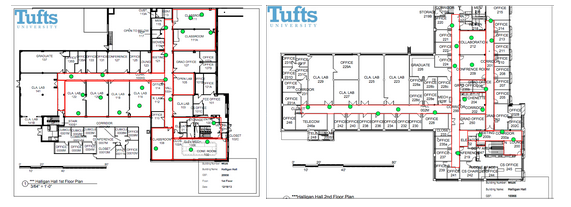
\includegraphics[width=0.5\textwidth]{testpoints}
   \caption{Test points on Halligan Floor 1 (left) and Floor 2 (right); red boxes indicate accessible regions, and green dots indicate test points}
   \label{fig:test_points}
\end{figure}

The accuracy of our positioning algorithm is dependent on the number of scans the WD makes for each test point, as shown in Figure \ref{fig:composite_accuracy}. Increasing the number of scans beyond five does not significantly improve the performance of our algorithm; therefore, we choose to test our positioning application against FPs gathered with five scans.

\begin{figure}[t!]
  \centering
    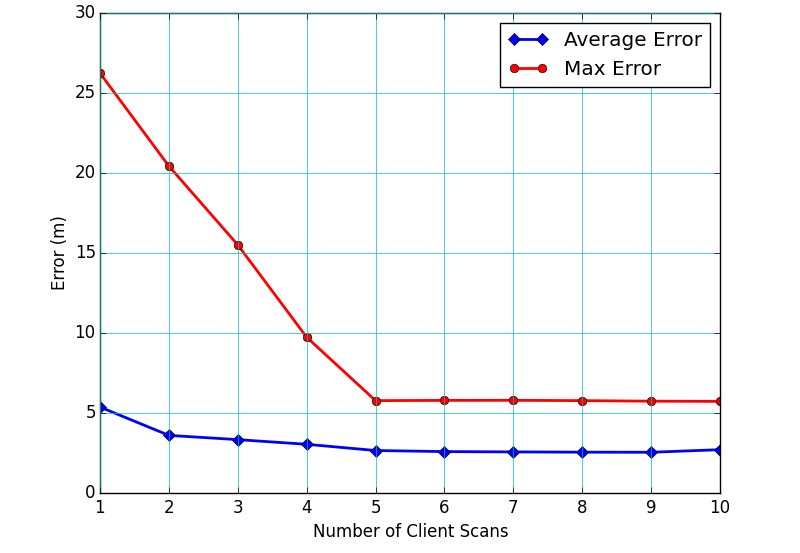
\includegraphics[width=0.5\textwidth]{pull_errors.png}
   \caption{Accuracy of the composite distance metric for various numbers of positioning scans}
   \label{fig:composite_accuracy}
\end{figure}

\subsection{Distance Metric Comparisons}
Figure \ref{fig:cdf_positioning_accuracy} shows the accuracy of our WKNN algorithm using the four distance metrics discussed in Section \ref{subsec:distance_metrics}. As the graph shows, the standard Euclidean distance metric performs significantly better than the Inverse Jaccard Coefficient, yielding average errors of 3.56m and 4.75m, respectively. Using the penalty-weighted Euclidean distance metric reduces the error to 2.87m. A linear combination of the two metrics only improves the performance slightly, bringing the average error to 2.78m. However, this linear combination reduces the maximum error to 9.70m, which is 21.1\% smaller than that of the penalty-weighted Euclidean distance metric alone. The composite distance metric is discussed in the next section.

\begin{table}[t!]
\renewcommand{\arraystretch}{1.3}
\caption{Distance Metric Accuracy}
\label{tab:table_distance_metric_accuracy}
\centering
\resizebox{\columnwidth}{!}{
\begin{tabular}{|c|c|c|}
\hline
\bfseries Distance Metric & Average Error ($m$) & Standard Deviation ($m$) \\
\hline
Inverse Jaccard Coefficient & 4.75  & 3.49\\
\hline
Euclidean distance	& 3.56   & 2.31\\
\hline
Penalty-Weighted Euclidean distance 	& 2.87   & 2.10\\
\hline
Linear Combination of $\sigma_{E'}$ and $\sigma_{J^{-1}}$ ($\sigma_{E' + J^{-1}}$)  	& 2.78   & 1.76\\
\hline
Composite Distance Metric& 2.66   & 1.44\\
\hline
\end{tabular}
}
\end{table}

\begin{figure}[t!]
  \centering
    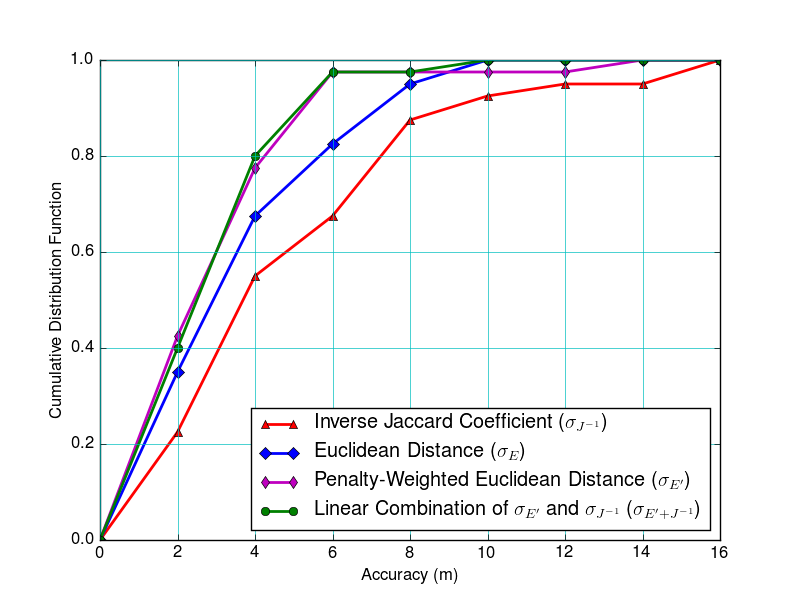
\includegraphics[width=0.5\textwidth]{distance_comparison.png}
    \caption{Cumulative distribution of positioning accuracy for various WKNN distance metrics (K=3)}
    \label{fig:cdf_positioning_accuracy}
\end{figure}


\subsection{Map-Aware Algorithm Refinement}

We add our Density-Penalizing Neighbor Weighting technique as a parameter to our composite distance metric ($\sigma_C$) in Equation \ref{eq:composite}. The accuracy of this metric can be seen in Figure \ref{fig:cdf_positioning_accuracy}. Overall, neighbor weighting decreases the average error from 2.78m to 2.66m. For points with less than 5m error, neighbor weighting increases the average error slightly, by 0.15m. However, the technique reduces the maximum error by 40.5\%, from 9.70m to 5.77m, and the average error of points with more than a 5m error by 50.1\%, from 7.12m to 3.55m. We consider this slight increase in average error for points with error less than 5m well worth the dramatic reduction in maximum error. The standard deviation of the error shown in Table \ref{tab:table_distance_metric_accuracy} also clearly reflects this improvement.\\	
\indent Figure \ref{fig:floor_preprocessing_effect} shows the our estimates of the effect of the floor detection preprocessing technique on runtime. For this calculation, we assume 100 locations per floor. This preprocessing does not improve runtime results in our testing environment, but our simulation indicates this technique would reduce positioning time by 39.1\%, from 6.89 seconds to 4.20 seconds, for a system with 100 floors. This time reduction results from the reduced number of penalty-weighted Euclidean distance calculations required once a floor has been identified. This performance improvement would be extremely significant in a large-scale commercial application.


\begin{figure}[t!]
  \centering
    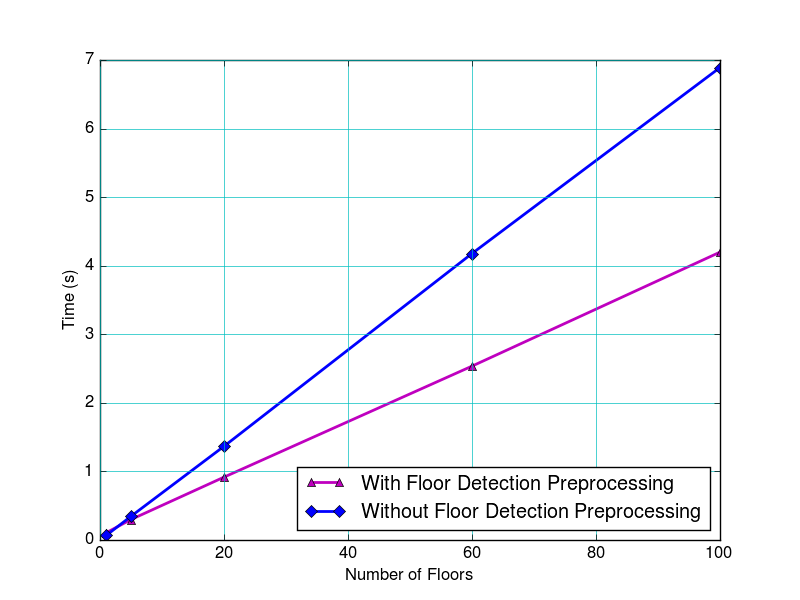
\includegraphics[width=0.5\textwidth]{time_comparison.png}
   \caption{Estimated effect of floor detection preprocessing technique on positioning time}
   \label{fig:floor_preprocessing_effect}
\end{figure}

\section{Discussion}
\indent Our positioning application has runtime and accuracy comparable to existing FP-based systems \cite{Liu}. Although there are fingerprinting positioning systems with higher accuracy, these often utilize application-specific hardware, whereas our application operates with consumer hardware and assumes no prior site information.\\
\indent Microsoft RADAR is an example of a system using KNN that achieved an average error of 3m to 5m using RF signals \cite{Bahl}. This system was implemented using one mapping device on a single floor that had three pre-arranged base stations. Our system achieves better accuracy with consumer hardware in a commercial-like setting. Subsequent iterations of RADAR incorporated continual user-tracking and multiple RSS maps for different environments, such as time of day \cite{Bahl2}. The same improvements could be applied to our system.\\
\indent Another very recent system uses improved double-peak Gaussian distributions and a probabilistic approach to determine position \cite{Chen}. This approach used a single device for mapping, and reported an average error of 1.5m. While this is a notably higher accuracy, the statistical analysis techniques used could be incorporated into our positioning application to improve accuracy.\\ 
\indent Beyond increasing scan numbers, several other methods and additional data could be incorporated to further improve our system accuracy, including the use of RSS standard deviation, multiple directions in site-survey, WD inertia, and prior knowledge of the site. These options are left as future work.

\section{Conclusion}
We implement a positioning system addressing many of the obstacles to widespread indoor positioning. We propose two novel metrics for use with the WKNN algorithm: Density-Penalizing Neighbor Weighting and Penalty-Weighted Euclidean Distance, as well an algorithm refinement for improved scalability: Floor Detection Preprocessing. Further improvement can be obtained by integrating other algorithm refinement techniques, such as Double Gaussian Distribution processing and the inclusion of user-feedback in the mapping process. Our positioning system is device-agnostic, able to serve multiple users, places no requirements on the site, and has an average accuracy of 2.66m, satisfying the requirements of most applications.

\section*{Acknowledgment}
We would like to thank Professor Chris Gregg of Tufts University for his advice and encouragement.


%----------------------------------------------------------------------------------------
%	REFERENCE LIST
%----------------------------------------------------------------------------------------

\begin{thebibliography}{99}


\bibitem{Lakmali} Lakmali, B.D.S. and D. Dias,
'Database Correlation for GSM Location in Outdoor and Indoor Environments',
\emph{4th Int'l Conf. on Information and Automation for Sustainability (ICIAFS).} Dec. 2008.

\bibitem{Liu} H, Liu, H. Darabi, P. Banerjee, and J. Li,
'Survey of Wireless Indoor Positioning Techniques and Systems',
\emph{ (Systems, Man, and Cybernetics, Part C: Applications and Reviews, IEEE Transactions on.} Nov. 2007.

\bibitem{Kokkinis} A. Kokkinis, M. Raspopoulos, L. Kanaris, A. Liotta and S. Stavrou,
'Map-aided fingerprint-based indoor positioning',
\emph{Personal Indoor and Mobile Radio Communications (PIMRC), 2013 IEEE 24th International Symposium on.} Sept. 2013.

\bibitem{Chaudhuri} K. Chaudhuri, D. Sanghi, and P. Bhagwat,
'Location Determination of a Mobile Device Using IEEE 802.11b Access Point Signals',
\emph{IEEE Xplore. IEEE}. Mar. 2003.

\bibitem{Bahl} P. Bahl and V. N. Padmanabhan,
'RADAR: An in-building RF-based user location and tracking system',
\emph{in Proc. IEEE INFOCOM.} Mar. 2000.

\bibitem{Fielding} R. Fielding,
'Architectural Styles and the Design of Network-based Software Architectures',
\emph{ (Unpublished Doctoral dissertation). University of California, Irvine.} 2000.

\bibitem{Sayad}  A. Sayed, A. Tarighat, and N. Khajehnouri,
'Challenges Faced in Developing Techniques for Accurate Wireless Location Information',
\emph{IEEE Signal Processing Magazine. IEEE, 1}. July 2005.
 
\bibitem{Sayad2} A. Sayed, A. Tarighat, and N. Khajehnouri,
'Performance Comparison of Indoor Positioning Techniques Based on Location Fingerprinting in Wireless Networks',
\emph{IEEE Xplore}. Jan. 2005.
 
\bibitem{Kemppi} P. Kemppi and S. Nousiainen,
'Database Correlation Method for Multi-System Positioning',
\emph{Vehicular Technology Conference (VTC) IEEE 63rd}. May 2006.

\bibitem{Dunbar} D. Dunbar and G. Humphreys,
'A Spatial Data Structure for Fast Poisson-Disk Sample Generation',
\emph{www.cs.virginia.edu. University of Virginia}. Jan. 2006.

\bibitem{Machaj} J. Machaj,, P. Brida, and R. Piche,
'Rank Based Fingerprinting Algorithm for Indoor Positioning',
\emph{Int'l Conf. on Indoor Positioning and Indoor Navigation (IPIN), Guimaraes, Portugal}. September 2011.

\bibitem{Bahl2} P. Bahl and V. N. Padmanabhan,
'Enhancements to the RADAR user location and tracking system',
\emph{Microsoft Corporation}. Feb. 2000.

\bibitem{Chen} L. Chen, B. Li, K. Zhao, C. Rizos, and Z. Zheng,
'An Improved Algorithm to Generate a Wi-Fi Fingerprint Database for Indoor Positioning',
\emph{Sensors (Basel, Switzerland). Molecular Diversity Preservation International (MDPI)}. Aug. 2013.


\end{thebibliography}

\end{document}


